
%{{第三十七回}}{第三十七回}}

\chapter{秋爽斋偶结海棠社\hspace{.5em}蘅芜苑夜拟菊花题}

{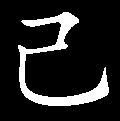
\includegraphics[width=3mm]{../Images/00003}美人用别号,亦新奇花样,且韵且雅,呼去觉满口生香。结社出自探春意,作者已伏下回``兴利除弊''之文也。}

{此回才放笔写诗、写词、作札,看他诗复诗、词复词、札又札,总不相犯。}

{湘云,诗客也,前回写之。其今才起社,后用不即不离闲人数语数折,仍归社中。何巧活之笔如此?}

{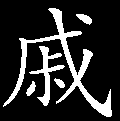
\includegraphics[width=3mm]{../Images/00005}海棠名诗社,林史傲秋闺。纵有才八斗,不如富贵儿。}

这年贾政又点了学差,择于八月二十日起身。是日拜过宗祠及贾母起身,宝玉诸子弟等送至洒泪亭。

却说贾政出门去后,外面诸事不能多记。\href{../Text/part0041_split_000.html\#lnkback_1_a}{\textsuperscript{①}}单表宝玉每日在园中任意纵性的旷荡,真把光阴虚度,岁月空添。这日正无聊之际,只见翠墨进来,手里拿着一副花笺送与他。宝玉因道:``可是我忘了,才说要瞧瞧三妹妹去的,可好些了,你偏走来。''翠墨道:``姑娘好了,今儿也不吃药了,不过是凉着一点儿。''宝玉听说,便展开花笺看时,上面写道:

娣探谨奉

二兄文几:前夕新霁,月色如洗,因惜清景难逢,讵忍就卧,时漏已三转,犹徘徊于桐槛之下,未防风露所欺,致获采薪之患。昨蒙亲劳抚嘱,复又数遣侍儿问切,兼以鲜荔并真卿墨迹见赐,何痌瘝惠爱之深哉!今因伏几凭床处默之时,因思及历来古人中处名攻利敌之场,犹置一些山滴水之区,远招近揖,投辖攀辕,务结二三同志盘桓于其中,或竖词坛,或开吟社,虽一时之偶兴,遂成千古之佳谈。娣虽不才,窃同叨栖处于泉石之间,而兼慕薛林之技。风庭月榭,惜未宴集诗人;帘杏溪桃,或可醉飞吟盏。孰谓莲社之雄才,独许须眉;直以东山之雅会,让余脂粉。若蒙棹雪而来,娣则扫花以待。此谨奉。

宝玉看了,不觉喜的拍手笑道:``倒是三妹妹的高雅,我如今就去商议。''一面说,一面就走,翠墨跟在后面。

刚到了沁芳亭,只见园中后门上值日的婆子手里拿着一个字帖走来,见了宝玉,便迎上去,口内说道:``芸哥儿请安,在后门只等着,叫我送来的。''宝玉打开看时,写道是:

不肖男芸恭请

父亲大人万福金安。男思自蒙天恩,认于膝下,日夜思一孝顺,竟无可孝顺之处。前因买办花草,上托大人金福,竟认得许多花儿匠,{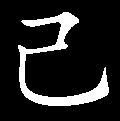
\includegraphics[width=3mm]{../Images/00003}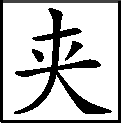
\includegraphics[width=3mm]{../Images/00012}\footnotesize \kaishu 直欲喷饭,真好新鲜文字。}并认得许多名园。因忽见有白海棠一种,不可多得。故变尽方法,只弄得两盆。大人若视男是亲男一般,{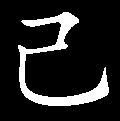
\includegraphics[width=3mm]{../Images/00003}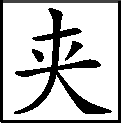
\includegraphics[width=3mm]{../Images/00012}\footnotesize \kaishu 皆千古未有之奇文,初读令人不解,思之则喷饭。}便留下赏玩。因天气暑热,恐园中姑娘们不便,故不敢面见。奉书恭启,并叩台安。男芸跪书。{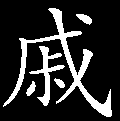
\includegraphics[width=3mm]{../Images/00005}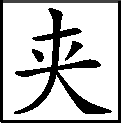
\includegraphics[width=3mm]{../Images/00012}\footnotesize \kaishu 一笑。 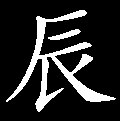
\includegraphics[width=3mm]{../Images/00009}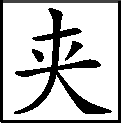
\includegraphics[width=3mm]{../Images/00012}\footnotesize \kaishu 接连二启,字句因人而施,诚作者之妙。}

宝玉看了,笑道:``独他来了,还有什么人?''婆子道:``还有两盆花儿。''宝玉道:``你出去说,我知道了,难为他想着。你便把花儿送到我屋里去就是了。''一面说,一面同翠墨往秋爽斋来,只见宝钗、黛玉、迎春、惜春已都在那里了。{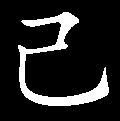
\includegraphics[width=3mm]{../Images/00003}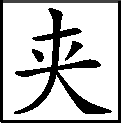
\includegraphics[width=3mm]{../Images/00012}\footnotesize \kaishu 却因芸之一字工夫,已将诸艳请来,省却多少闲文。不然必云如何请如何来,则必至有犯宝玉,终成重复之文矣。}

众人见他进来,都笑说:``又来了一个。''探春笑道:``我不算俗,偶然起个念头,写了几个帖儿试一试,谁知一招皆到。''宝玉笑道:``可惜迟了,早该起个社的。''黛玉道:``你们只管起社,可别算上我,我是不敢的。''迎春笑道:``你不敢谁还敢呢。''{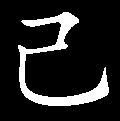
\includegraphics[width=3mm]{../Images/00003}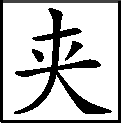
\includegraphics[width=3mm]{../Images/00012}\footnotesize \kaishu 必得如此方是妙文。若也如宝玉说兴头话,则不是黛玉矣。}宝玉道:``这是一件正经大事,大家鼓舞起来,不要你谦我让的。各有主意自管说出来大家平章。{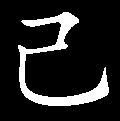
\includegraphics[width=3mm]{../Images/00003}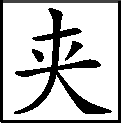
\includegraphics[width=3mm]{../Images/00012}\footnotesize \kaishu ``这是正经大事''已妙,且曰``平章'',更妙!的是宝玉口角。}宝姐姐也出个主意,林妹妹也说个话儿。''宝钗道:``你忙什么,人还不全呢。''{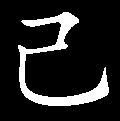
\includegraphics[width=3mm]{../Images/00003}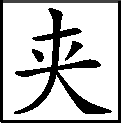
\includegraphics[width=3mm]{../Images/00012}\footnotesize \kaishu 妙!宝钗自有主见,真不诬也。}一语未了,李纨也来了,进门笑道:``雅的紧!要起诗社,我自荐我掌坛。前儿春天我原有这个意思的。我想了一想,我又不会作诗,瞎乱些什么,因而也忘了,就没有说得。既是三妹妹高兴,我就帮你作兴起来。''{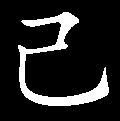
\includegraphics[width=3mm]{../Images/00003}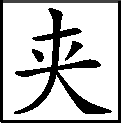
\includegraphics[width=3mm]{../Images/00012}\footnotesize \kaishu 看他又是一篇文字,分叙单传之法也。}

黛玉道:``既然定要起诗社,咱们都是诗翁了,先把这些姐妹叔嫂的字样改了才不俗。''{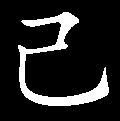
\includegraphics[width=3mm]{../Images/00003}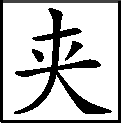
\includegraphics[width=3mm]{../Images/00012}\footnotesize \kaishu 看他写黛玉,真可人也。}李纨道:``极是,何不大家起个别号,彼此称呼则雅。{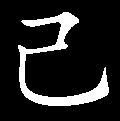
\includegraphics[width=3mm]{../Images/00003}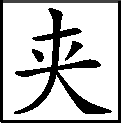
\includegraphics[width=3mm]{../Images/00012}\footnotesize \kaishu 未起诗社,先起别号。}我是定了`稻香老农',再无人占的。''{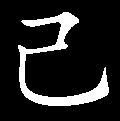
\includegraphics[width=3mm]{../Images/00003}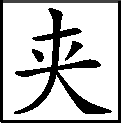
\includegraphics[width=3mm]{../Images/00012}\footnotesize \kaishu 最妙!一个花样。}探春笑道:``我就是`秋爽居士'罢。''宝玉道:``\,`居士'、`主人'到底不恰,且又瘰赘。这里梧桐芭蕉尽有,或指梧桐芭蕉起个倒好。''探春笑道:``有了,我最喜芭蕉,就称`蕉下客'罢。''众人都道别致有趣。黛玉笑道:``你们快牵了他去,炖了脯子吃酒。''众人不解。黛玉笑道:``古人曾云`蕉叶覆鹿'。他自称`蕉下客',可不是一只鹿了?快做了鹿脯来。''众人听了都笑起来。探春因笑道:``你别忙中使巧话来骂人,我已替你想了个极当的美号了。''又向众人道:``当日娥皇女英洒泪在竹上成斑,故今斑竹又名湘妃竹。如今他住的是潇湘馆,他又爱哭,将来他想林姐夫,那些竹子也是要变成斑竹的。以后都叫他作`潇湘妃子'就完了。''大家听说,都拍手叫妙。林黛玉低了头方不言语。{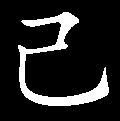
\includegraphics[width=3mm]{../Images/00003}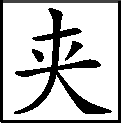
\includegraphics[width=3mm]{../Images/00012}\footnotesize \kaishu 妙极趣极!所谓``夫人必自侮然后人侮之'',看因一谑便勾出一美号来,何等妙文哉!另一花样。}李纨笑道:``我替薛大妹妹也早已想了个好的,也只三个字。''惜春迎春都问是什么。{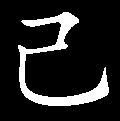
\includegraphics[width=3mm]{../Images/00003}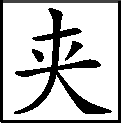
\includegraphics[width=3mm]{../Images/00012}\footnotesize \kaishu 妙文!迎春惜春固不能答言,然不便置之不叙,故插他二人问。试思近日诸豪宴集雄语伟辩之时,座上或有一二愚夫不敢接谈,然偏好问,亦真可厌之事也。}李纨道:``我是封他为`蘅芜君'了,不知你们如何。''探春笑道:``这个封号极好。''宝玉道:``我呢?你们也替我想一个。''{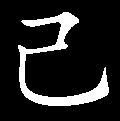
\includegraphics[width=3mm]{../Images/00003}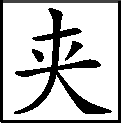
\includegraphics[width=3mm]{../Images/00012}\footnotesize \kaishu 必有是问。}宝钗笑道:``你的号早有了,`无事忙'三字恰当的很。''{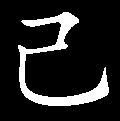
\includegraphics[width=3mm]{../Images/00003}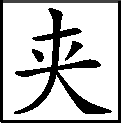
\includegraphics[width=3mm]{../Images/00012}\footnotesize \kaishu 真恰当,形容的尽。}李纨道:``你还是你的旧号`绛洞花王'就好。''{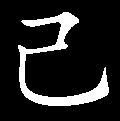
\includegraphics[width=3mm]{../Images/00003}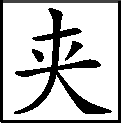
\includegraphics[width=3mm]{../Images/00012}\footnotesize \kaishu 妙极!又点前文。通部中从头至末,前文已过者恐去之冷落,使人忘怀,得便一点。未来者恐来之突然,或先伏一线。皆行文之妙诀也。}宝玉笑道:``小时候干的营生,还提他作什么。''{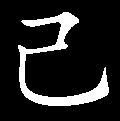
\includegraphics[width=3mm]{../Images/00003}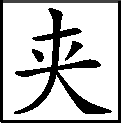
\includegraphics[width=3mm]{../Images/00012}\footnotesize \kaishu 赧言如闻,不知大时又有何营生。}探春道:``你的号多的很,又起什么。我们爱叫你什么,你就答应着就是了。''{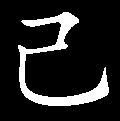
\includegraphics[width=3mm]{../Images/00003}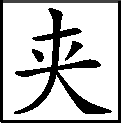
\includegraphics[width=3mm]{../Images/00012}\footnotesize \kaishu 更妙!若只管挨次一个一个乱起,则成何文字?◇另一花样。}宝钗道:``还得我送你个号罢。有最俗的一个号,却于你最当。天下难得的是富贵,又难得的是闲散,这两样再不能兼有,不想你兼有了,就叫你`富贵闲人'也罢了。''宝玉笑道:``当不起,当不起,倒是随你们混叫去罢。''李纨道:``二姑娘四姑娘起个什么号?''迎春道:``我们又不大会诗,白起个号作什么?''{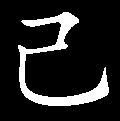
\includegraphics[width=3mm]{../Images/00003}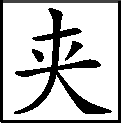
\includegraphics[width=3mm]{../Images/00012}\footnotesize \kaishu 假斯文守钱虏来看这句。}探春道:``虽如此,也起个才是。''宝钗道:``他住的是紫菱洲,就叫他`菱洲';四丫头在藕香榭,就叫他`藕榭'就完了。''

李纨道:``就是这样好。但序齿我大,你们都要依我的主意,管情说了大家合意。我们七个人起社,我和二姑娘四姑娘都不会作诗,须得让出我们三个人去。我们三个各分一件事。''探春笑道:``已有了号,还只管这样称呼,不如不有了。以后错了,也要立个罚约才好。''李纨道:``立定了社,再定罚约。我那里地方大,竟在我那里作社。我虽不能作诗,这些诗人竟不厌俗客,我作个东道主人,我自然也清雅起来了。若是要推我作社长,我一个社长自然不够,必要再请两位副社长,就请菱洲藕榭二位学究来,一位出题限韵,一位誊录监场。亦不可拘定了我们三个人不作,若遇见容易些的题目韵脚,我们也随便作一首。你们四个却是要限定的。若如此便起,若不依我,我也不敢附骥了。''迎春惜春本性懒于诗词,又有薛林在前,听了这话便深合己意,二人皆说:``极是。''探春等也知此意,见他二人悦服,也不好强,只得依了。因笑道:``这话也罢了,只是自想好笑,好好的我起了个主意,反叫你们三个来管起我来了。''宝玉道:``既这样,咱们就往稻香村去。''李纨道:``都是你忙,今日不过商议了,等我再请。''宝钗道:``也要议定几日一会才好。''探春道:``若只管会的多,又没趣了。一月之中,只可两三次才好。''宝钗点头道:``一月只要两次就够了。拟定日期,风雨无阻。除这两日外,倘有高兴的,他情愿加一社的,或情愿到他那里去,或附就了来,亦可使得,岂不活泼有趣。''众人都道:``这个主意更好。''

探春道:``只是原系我起的意,我须得先作个东道主人,方不负我这兴。''李纨道:``既这样说,明日你就先开一社如何?''探春道:``明日不如今日,此刻就很好。你就出题,菱洲限韵,藕榭监场。''迎春道:``依我说,也不必随一人出题限韵,竟是拈阄公道。''李纨道:``方才我来时,看见他们抬进两盆白海棠来,倒是好花。你们何不就咏起他来?''{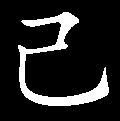
\includegraphics[width=3mm]{../Images/00003}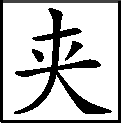
\includegraphics[width=3mm]{../Images/00012}\footnotesize \kaishu 真正好题目。妙在未起诗社先得了题目。}迎春道:``都还未赏,先倒作诗。''宝钗道:``不过是白海棠,又何必定要见了才作。古人的诗赋,也不过都是寄兴写情耳。若都是等见了作,如今也没这些诗了。''{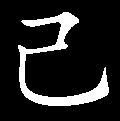
\includegraphics[width=3mm]{../Images/00003}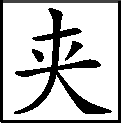
\includegraphics[width=3mm]{../Images/00012}\footnotesize \kaishu 真诗人语。}迎春道:``既如此,待我限韵。''说着,走到书架前抽出一本诗来,随手一揭,这首竟是一首七言律,递与众人看了,都该作七言律。迎春掩了诗,又向一个小丫头道:``你随口说一个字来。''那丫头正倚门立着,便说了个``门''字。迎春笑道:``就是门字韵,`十三元'了。头一个韵定要这`门'字。''说着,又要了韵牌匣子过来,抽出``十三元''一屉,又命那小丫头随手拿四块。那丫头便拿了``盆''``魂''``痕''``昏''四块来。宝玉道:``这`盆'`门'两个字不大好作呢!''

待书一样预备下四份纸笔,便都悄然各自思索起来。独黛玉或抚梧桐,或看秋色,或又和丫鬟们嘲笑。{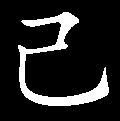
\includegraphics[width=3mm]{../Images/00003}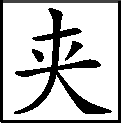
\includegraphics[width=3mm]{../Images/00012}\footnotesize \kaishu 看他单写黛玉。}迎春又令丫鬟炷了一支``梦甜香''。原来这``梦甜香''只有三寸来长,有灯草粗细,以其易烬,故以此烬为限,如香烬未成便要罚。{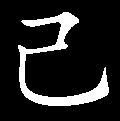
\includegraphics[width=3mm]{../Images/00003}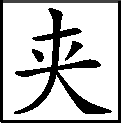
\includegraphics[width=3mm]{../Images/00012}\footnotesize \kaishu 好香!专能撰此新奇字样。}一时探春便先有了,自提笔写出,又改抹了一回,递与迎春。因问宝钗:``蘅芜君,你可有了?''宝钗道:``有却有了,只是不好。''宝玉背着手,在回廊上踱来踱去,因向黛玉说道:``你听,他们都有了。''黛玉道:``你别管我。''宝玉又见宝钗已誊写出来,因说道:``了不得!香只剩了一寸了,我才有了四句。''又向黛玉道:``香就完了,只管蹲了那潮地下作什么?''黛玉也不理。宝玉道:``我可顾不得你了,好歹也写出来罢。''说着也走在案前写了。李纨道:``我们要看诗了,若看完了还不交卷是必罚的。''宝玉道:``稻香老农虽不善作却善看,又最公道,{\includegraphics[width=3mm]{../Images/00003}\includegraphics[width=3mm]{../Images/00012}\footnotesize \kaishu 理岂不公。}你就评阅优劣,我们都服的。''众人都道:``自然。''于是先看探春的稿上写道是:

咏白海棠 {限门盆魂痕昏}

斜阳寒草带重门,苔翠盈铺雨后盆。

玉是精神难比洁,雪为肌骨易消魂。

芳心一点娇无力,倩影三更月有痕。

莫谓缟仙能羽化,多情伴我咏黄昏。

大家看了,称赏一回,又看宝钗的道:

珍重芳姿昼掩门,{{\includegraphics[width=3mm]{../Images/00003}\includegraphics[width=3mm]{../Images/00012}\footnotesize \kaishu 宝钗诗全是自写身份,讽刺时事。只以品行为先,才技为末。纤巧流荡之词、绮靡}秾{艳之语,一洗皆尽。非不能也,屑而不为也。最恨近日小说中,一百美人诗词语气,只得一个艳稿。}}自携手瓮灌苔盆。

胭脂洗出秋阶影,冰雪招来露砌魂。{\includegraphics[width=3mm]{../Images/00003}\includegraphics[width=3mm]{../Images/00012}\footnotesize \kaishu 看他清洁自厉,终不肯作一轻浮语。}

淡极始知花更艳,{\includegraphics[width=3mm]{../Images/00003}\includegraphics[width=3mm]{../Images/00012}\footnotesize \kaishu 好极!高情巨眼能几人哉!正``一鸟不鸣山更幽''也。}愁多焉得玉无痕。{\includegraphics[width=3mm]{../Images/00003}\includegraphics[width=3mm]{../Images/00012}\footnotesize \kaishu 看他讽刺林、宝二人,省手。}

欲偿白帝凭清洁,{\includegraphics[width=3mm]{../Images/00003}\includegraphics[width=3mm]{../Images/00012}\footnotesize \kaishu 看他收到自己身上来,是何等身份。}不语婷婷日又昏。

李纨笑道:``到底是蘅芜君。''说着又看宝玉的,道是:

秋容浅淡映重门,七节攒成雪满盆。

出浴太真冰作影,捧心西子玉为魂。

晓风不散愁千点,{\includegraphics[width=3mm]{../Images/00003}\includegraphics[width=3mm]{../Images/00012}\footnotesize \kaishu 这句直是自己一生心事。}宿雨还添泪一痕。{\includegraphics[width=3mm]{../Images/00003}\includegraphics[width=3mm]{../Images/00012}\footnotesize \kaishu 妙在终不忘黛玉。}

独倚画栏如有意,清砧怨笛送黄昏。{\includegraphics[width=3mm]{../Images/00003}\includegraphics[width=3mm]{../Images/00012}\footnotesize \kaishu 宝玉再细心作,只怕还有好的。只是一心挂着黛玉,故平妥不警也。}

大家看了,宝玉说探春的好,李纨才要推宝钗这诗有身分,因又催黛玉。黛玉道:``你们都有了?''说着提笔一挥而就,掷与众人。李纨等看他写道是:

半卷湘帘半掩门,{\includegraphics[width=3mm]{../Images/00003}\includegraphics[width=3mm]{../Images/00012}\footnotesize \kaishu 且不说花,且说看花的人,起的突然别致。}碾冰为土玉为盆。{\includegraphics[width=3mm]{../Images/00003}\includegraphics[width=3mm]{../Images/00012}\footnotesize \kaishu 极妙!料定他自与别人不同。}

看了这句,宝玉先喝起彩来,只说``从何处想来!''又看下面道:

偷来梨蕊三分白,借得梅花一缕魂。

众人看了也都不禁叫好,说``果然比别人又是一样心肠。''又看下面道是:

月窟仙人缝缟袂,秋闺怨女拭啼痕。{\includegraphics[width=3mm]{../Images/00003}\includegraphics[width=3mm]{../Images/00012}\footnotesize \kaishu 虚敲旁比,真逸才也。且不脱落自己。}

娇羞默默同谁诉,倦倚西风夜已昏。{\includegraphics[width=3mm]{../Images/00003}\includegraphics[width=3mm]{../Images/00012}\footnotesize \kaishu 看他终结道自己,一人是一人口气。逸才仙品固让颦儿,温雅沉着终是宝钗。今日之作宝玉自应居末。}

众人看了,都道是这首为上。李纨道:``若论风流别致,自是这首;若论含蓄浑厚,终让蘅稿。''探春道:``这评的有理,潇湘妃子当居第二。''李纨道:``怡红公子是压尾,你服不服?''宝玉道:``我的那首原不好了,这评的最公。''{\includegraphics[width=3mm]{../Images/00003}\includegraphics[width=3mm]{../Images/00012}\footnotesize \kaishu 话内细思,则似有不服先评之意。}又笑道:``只是蘅潇二首还要斟酌。''李纨道:``原是依我评论,不与你们相干,再有多说者必罚。''宝玉听说,只得罢了。李纨道:``从此后我定于每月初二、十六这两日开社,出题限韵都要依我。这其间你们有高兴的,你们只管另择日子补开,那怕一个月每天都开社,我只不管。只是到了初二、十六这两日,是必往我那里去。''宝玉道:``到底要起个社名才是。''探春道:``俗了又不好,特新了,刁钻古怪也不好。可巧才是海棠诗开端,就叫个海棠社罢。虽然俗些,因真有此事,也就不碍了。''说毕大家又商议了一回,略用些酒果,方各自散去。也有回家的,也有往贾母王夫人处去的。当下别人无话。{\includegraphics[width=3mm]{../Images/00003}\includegraphics[width=3mm]{../Images/00012}\footnotesize \kaishu 一路总不大写薛、林兴头,可见他二人并不着意于此。◇不写薛、林,正是大手笔,独他二人长于诗,必使他二人为之则板腐矣。全是错综法。}

且说袭人{\includegraphics[width=3mm]{../Images/00003}\includegraphics[width=3mm]{../Images/00012}\footnotesize \kaishu 忽然写到袭人,真令人不解。看他如何终此诗社之文。}因见宝玉看了字贴儿便慌慌张张的同翠墨去了,也不知是何事。后来又见后门上婆子送了两盆海棠花来。袭人问是那里来的,婆子便将宝玉前一番缘故说了。袭人听说便命他们摆好,让他们在下房里坐了,自己走到自己房内秤了六钱银子封好,又拿了三百钱走来,都递与那两个婆子道:``这银子赏那抬花来的小子们,这钱你们打酒吃罢。''那婆子们站起来,眉开眼笑,千恩万谢的不肯受,见袭人执意不收,方领了。袭人又道:``后门上外头可有该班的小子们?''婆子忙应道:``天天有四个,原预备里面差使的。姑娘有什么差使,我们吩咐去。''袭人笑道:``有什么差使?今儿宝二爷要打发人到小侯爷家与史大姑娘送东西去,可巧你们来了,顺便出去叫后门小子们雇辆车来。回来你们就往这里拿钱,不用叫他们又往前头混碰去。''婆子答应着去了。

袭人回至房中,拿碟子盛东西与史湘云送去,{\includegraphics[width=3mm]{../Images/00003}\includegraphics[width=3mm]{../Images/00012}\footnotesize \kaishu 线头却牵出,观者犹不理会。◇不知是何碟何物,令人犯思夺。}却见槅子上碟槽空着。{\includegraphics[width=3mm]{../Images/00003}\includegraphics[width=3mm]{../Images/00012}\footnotesize \kaishu 妙极,细极!因此处系依古董式样抠成槽子,故无此件,此槽遂空。若忘却前文,此句不解。}因回头见晴雯、秋纹、麝月等都在一处做针黹,袭人问道:``这一个缠丝白玛瑙碟子那去了?''众人见问,都你看我我看你,都想不起来。半日,晴雯笑道:``给三姑娘送荔枝去的,还没送来呢。''袭人道:``家常送东西的家伙也多,巴巴的拿这个去。''晴雯道:``我何尝不也这样说。他说这个碟子配上鲜荔枝才好看。{\includegraphics[width=3mm]{../Images/00003}\includegraphics[width=3mm]{../Images/00012}\footnotesize \kaishu 自然好看,原该如此。可恨今之有一二好花者,不肯像景而用。}我送去,三姑娘见了也说好看,叫连碟子放着,就没带来。你再瞧,那槅子尽上头的一对联珠瓶还没收来呢。''

秋纹笑道:``提起瓶来,我又想起笑话。我们宝二爷说声孝心一动,也孝敬到二十分。因那日见园里桂花,折了两枝,原是自己要插瓶的,忽然想起来说,这是自己园里的才开的新鲜花,不敢自己先顽,巴巴的把那一对瓶拿下来,亲自灌水插好了,叫个人拿着,亲自送一瓶进老太太,又进一瓶与太太。谁知他孝心一动,连跟的人都得了福了。可巧那日是我拿去的。老太太见了这样,喜的无可无不可,见人就说:`到底是宝玉孝顺我,连一枝花儿也想的到。别人还只抱怨我疼他。'你们知道,老太太素日不大同我说话的,有些不入他老人家的眼的。那日竟叫人拿几百钱给我,说我可怜见的,生的单柔。这可是再想不到的福气。几百钱是小事,难得这个脸面。及至到了太太那里,太太正和二奶奶、赵姨奶奶、周姨奶奶好些人翻箱子,找太太当日年轻的颜色衣裳,不知给那一个。一见了,连衣裳也不找了,且看花儿。又有二奶奶在旁边凑趣儿,夸宝玉又是怎么孝敬,又是怎样知好歹,有的没的说了两车话。当着众人,太太自为又增了光,堵了众人的嘴。太太越发喜欢了,现成的衣裳就赏了我两件。衣裳也是小事,年年横竖也得,却不像这个彩头。''

晴雯笑道:``呸!没见世面的小蹄子!那是把好的给了人,挑剩下的才给你,你还充有脸呢。''秋纹道:``凭他给谁剩的,到底是太太的恩典。''晴雯道:``要是我,我就不要。若是给别人剩下的给我,也罢了。一样这屋里的人,难道谁又比谁高贵些?把好的给他,剩下的才给我,我宁可不要,冲撞了太太,我也不受这口软气。''秋纹忙问:``给这屋里谁的?我因为前儿病了几天,家去了,不知是给谁的。好姐姐,你告诉我知道知道。''晴雯道:``我告诉了你,难道你这会退还太太去不成?''秋纹笑道:``胡说。我白听了喜欢喜欢。那怕给这屋里的狗剩下的,我只领太太的恩典,也不犯管别的事。''众人听了都笑道:``骂的巧,可不是给了那西洋花点子哈巴儿了。''袭人笑道:``你们这起烂了嘴的!得了空就拿我取笑打牙儿。一个个不知怎么死呢。''秋纹笑道:``原来姐姐得了,我实在不知道。我陪个不是罢。''袭人笑道:``少轻狂罢。你们谁取了碟子来是正经。''{\includegraphics[width=3mm]{../Images/00003}\includegraphics[width=3mm]{../Images/00012}\footnotesize \kaishu 看他忽然夹写女儿喁喁一段,总不脱落正事。所谓此书一回是两段,两段中却有无限事体,或有一语透至下回者,或有反补上回者,错综穿插,从不一气直起直泻,至终为了。}麝月道:``那瓶得空儿也该收来了。老太太屋里还罢了,太太屋里人多手杂。别人还可以,赵姨奶奶一伙的人见是这屋里的东西,又该使黑心弄坏了才罢。太太也不大管这些,不如早些收来正经。''晴雯听说,便掷下针黹道:``这话倒是,等我取去。''秋纹道:``还是我取去罢,你取你的碟子去。''晴雯笑道:``我偏取一遭儿去。是巧宗儿你们都得了,难道不许我得一遭儿?''麝月笑道:``通共秋丫头得了一遭儿衣裳,那里今儿又巧,你也遇见找衣裳不成。''晴雯冷笑道:``虽然碰不见衣裳,或者太太看见我勤谨,一个月也把太太的公费里分出二两银子来给我,也定不得。''说着,又笑道:``你们别和我装神弄鬼的,什么事我不知道。''一面说,一面往外跑了。秋纹也同他出来,自去探春那里取了碟子来。

袭人打点齐备东西,叫过本处的一个老宋妈妈来,{\includegraphics[width=3mm]{../Images/00003}\includegraphics[width=3mm]{../Images/00012}\footnotesize \kaishu ``宋'',送也。随事生文,妙!}向他说道:``你先好生梳洗了,换了出门的衣裳来,如今打发你与史姑娘送东西去。''那宋嬷嬷道:``姑娘只管交给我,有话说与我,我收拾了就好一顺去的。''袭人听说,便端过两个小掐丝盒子来。先揭开一个,里面装的是红菱和鸡头{\includegraphics[width=3mm]{../Images/00003}\includegraphics[width=3mm]{../Images/00012}\footnotesize \kaishu 妙!}两样鲜果;又那一个是一碟子桂花糖蒸新栗粉糕。又说道:``这都是今年咱们这里园里新结的果子,宝二爷送来与姑娘尝尝。再前日姑娘说这玛瑙碟子好,姑娘就留下顽罢。{\includegraphics[width=3mm]{../Images/00003}\includegraphics[width=3mm]{../Images/00012}\footnotesize \kaishu 妙!隐这一件公案。余想袭人必要玛瑙碟子盛去,何必娇奢轻发如是耶?因有此一案,则无怪矣。}这绢包儿里头是姑娘上日叫我作的活计,姑娘别嫌粗糙,能着用罢。替我们请安,替二爷问好就是了。''宋嬷嬷道:``宝二爷不知还有什么说的,姑娘再问问去,回来又别说忘了。''袭人因问秋纹:``方才可见在三姑娘那里?''秋纹道:``他们都在那里商议起什么诗社呢,又都作诗。想来没话,你只去罢。''宋嬷嬷听了,便拿了东西出去,另外穿戴了。袭人又嘱咐他:``从后门出去,有小子和车等着呢。''宋妈去后,不在话下。

一时,宝玉回来,先忙着看了一回海棠,至房内告诉袭人起诗社的事。袭人也把打发宋妈妈与史湘云送东西去的话告诉了宝玉。宝玉听了,拍手道:``偏忘了他。我自觉心里有件事,只是想不起来,亏你提起来,正要请他去。这诗社里若少了他还有什么意思。''袭人劝道:``什么要紧,不过玩意儿。他比不得你们自在,家里又作不得主儿。告诉他,他要来又由不得他;不来,他又牵肠挂肚的,没的叫他不受用。''宝玉道:``不妨事,我回老太太打发人接他去。''正说着,宋妈妈已经回来,回复道生受,与袭人道乏,又说:``问二爷作什么呢,我说和姑娘们起什么诗社作诗呢。史姑娘说,他们作诗也不告诉他去,急的了不的。''宝玉听了立身便往贾母处来,立逼着叫人接去。贾母因说:``今儿天晚了,明日一早再去。''宝玉只得罢了,回来闷闷的。

次日一早,便又往贾母处来催逼人接去。直到午后,史湘云才来,宝玉方放了心,见面时就把始末原由告诉他,又要与他诗看。李纨等因说道:``且别给他诗看,先说与他韵。他后来,先罚他和了诗:若好,便请入社;若不好,还要罚他一个东道再说。''史湘云道:``你们忘了请我,我还要罚你们呢。就拿韵来,我虽不能,只得勉强出丑。容我入社,扫地焚香我也情愿。''众人见他这般有趣,越发喜欢,都埋怨昨日怎么忘了他,遂忙告诉他韵。史湘云一心兴头,等不得推敲删改,一面只管和人说着话,心内早已和成,即用随便的纸笔录出,{\includegraphics[width=3mm]{../Images/00003}\includegraphics[width=3mm]{../Images/00012}\footnotesize \kaishu 可见越是好文字,不管怎样就有了。越用工夫,越讲究笔墨,终成涂鸦。}先笑说道:``我却依韵和了两首,{\includegraphics[width=3mm]{../Images/00003}\includegraphics[width=3mm]{../Images/00012}\footnotesize \kaishu 更奇!想前四律已将形容尽矣,一首犹恐重犯,不知二首又从何处着笔。}好歹我却不知,不过应命而已。''说着递与众人。众人道:``我们四首也算想绝了,再一首也不能了。你倒弄了两首,那里有许多话说,必要重了我们。''一面说,一面看时,只见那两首诗写道:

其一

神仙昨日降都门,{\includegraphics[width=3mm]{../Images/00003}\includegraphics[width=3mm]{../Images/00012}\footnotesize \kaishu 落想便新奇,不落彼四套。}种得蓝田玉一盆。{\includegraphics[width=3mm]{../Images/00003}\includegraphics[width=3mm]{../Images/00012}\footnotesize \kaishu 好!``盆''字押得更稳,总不落彼{(三)}{[}四{]}套。}

自是霜娥偏爱冷,{\includegraphics[width=3mm]{../Images/00003}\includegraphics[width=3mm]{../Images/00012}\footnotesize \kaishu 又不脱自己将来形景。}非关倩女亦离魂。

秋阴捧出何方雪,{\includegraphics[width=3mm]{../Images/00003}\includegraphics[width=3mm]{../Images/00012}\footnotesize \kaishu 拍案叫绝!压倒群芳在此一句。}雨渍添来隔宿痕。

却喜诗人吟不倦,岂令寂寞度朝昏。{\includegraphics[width=3mm]{../Images/00003}\includegraphics[width=3mm]{../Images/00012}\footnotesize \kaishu 真好!}

其二

蘅芷阶通萝薜门,也宜墙角也宜盆。{\includegraphics[width=3mm]{../Images/00003}\includegraphics[width=3mm]{../Images/00012}\footnotesize \kaishu 更好!}

花因喜洁难寻偶,人为悲秋易断魂。

玉烛滴干风里泪,晶帘隔破月中痕。

幽情欲向嫦娥诉,无奈虚廊夜色昏。{\includegraphics[width=3mm]{../Images/00003}\includegraphics[width=3mm]{../Images/00012}\footnotesize \kaishu 二首真可压卷。◇诗是好诗,文是奇奇怪怪之文,总令人想不到,忽有二首来压卷。}

众人看一句,惊讶一句,看到了,赞到了,都说:``这个不枉作了海棠诗,真该要起海棠社了。''史湘云道:``明日先罚我个东道,就让我先邀一社可使得?''众人道:``这更妙了。''因又将昨日的与他评论了一回。

至晚,宝钗将湘云邀往蘅芜苑安歇去。湘云灯下计议如何设东拟题。宝钗听他说了半日,皆不妥当,{\includegraphics[width=3mm]{../Images/00003}\includegraphics[width=3mm]{../Images/00012}\footnotesize \kaishu 却于此刻方写宝钗。}因向他说道:``既开社,便要作东。虽然是顽意儿,也要瞻前顾后,又要自己便宜,又要不得罪了人,然后方大家有趣。你家里你又作不得主,一个月通共那几串钱,你还不够盘缠呢。这会子又干这没要紧的事,你婶子听见了,越发抱怨你了。况且你就都拿出来,做这个东道也是不够。难道为这个家去要不成?还是往这里要呢?''一席话提醒了湘云,倒踌蹰起来。宝钗道:``这个我已经有个主意。我们当铺里有个伙计,他家田上出的很好的肥螃蟹,前儿送了几斤来。现在这里的人,从老太太起连上园里的人,有多一半都是爱吃螃蟹的。前日姨娘还说要请老太太在园里赏桂花吃螃蟹,因为有事还没有请呢。你如今且把诗社别提起,只管普通一请。等他们散了,咱们有多少诗作不得的。我和我哥哥说,要几篓极肥极大的螃蟹来,再往铺子里取上几坛好酒,再备上四五桌果碟,岂不又省事又大家热闹了。''湘云听了,心中自是感服,极赞他想的周到。宝钗又笑道:``我是一片真心为你的话。你千万别多心,想着我小看了你,咱们两个就白好了。你若不多心,我就好叫他们办去的。''湘云忙笑道:``好姐姐,你这样说,倒多心待我了。凭他怎么糊涂,连个好歹也不知,还成个人了?我若不把姐姐当亲姐姐一样看,上回那些家常话烦难事也不肯尽情告诉你了。''宝钗听说,便叫一个婆子来:``出去和大爷说,依前日的大螃蟹要几篓来,明日饭后请老太太姨娘赏桂花。你说大爷好歹别忘了,我今儿已请下人了。''{\includegraphics[width=3mm]{../Images/00003}\includegraphics[width=3mm]{../Images/00012}\footnotesize \kaishu 必得如此叮咛,阿呆兄方记得。}那婆子出去说明,回来无话。

这里宝钗又向湘云道:``诗题也不要过于新巧了。你看古人诗中那些刁钻古怪的题目和那极险的韵了,若题过于新巧,韵过于险,再不得有好诗,终是小家气。诗固然怕说熟话,更不可过于求生,只要头一件立意清新,自然措词就不俗了。究竟这也算不得什么,还是纺绩针黹是你我的本等。一时闲了,倒是于你我深有益的书看几章是正经。''

湘云只答应着,因笑道:``我如今心里想着,昨日作了海棠诗,我如今要作个菊花诗如何?''宝钗道:``菊花倒也合景,只是前人太多了。''湘云道:``我也是如此想着,恐怕落套。''宝钗想了一想,说道:``有了,如今以菊花为宾,以人为主,竟拟出几个题目来,都是两个字:一个虚字,一个实字,实字便用`菊'字,虚字就用通用门的。如此又是咏菊,又是赋事,前人也没作过,也不能落套。赋景咏物两关着,又新鲜,又大方。''湘云笑道:``这却很好。只是不知用何等虚字才好。你先想一个我听听。''宝钗想了一想,笑道:``《菊梦》就好。''湘云笑道:``果然好。我也有一个,《菊影》可使得?''宝钗道:``也罢了。只是也有人作过,若题目多,这个也夹的上。我又有了一个。''湘云道:``快说出来。''宝钗道:``《问菊》如何?''湘云拍案叫妙,因接说道:``我也有了,《访菊》如何?''宝钗也赞有趣,因说道:``越性拟出十个来,写上再来。''说着,二人研墨蘸笔,湘云便写,宝钗便念,一时凑了十个。湘云看了一遍,又笑道:``十个还不成幅,越性凑成十二个便全了,也如人家的字画册页一样。''宝钗听说,又想了两个,一共凑成十二。又说道:``既这样,越性编出他个次序先后来。''湘云道:``如此更妙,竟弄成个菊谱了。''宝钗道:``起首是《忆菊》;忆之不得,故访,第二是《访菊》;访之既得,便种,第三是《种菊》;种既盛开,故相对而赏,第四是《对菊》;相对而兴有馀,故折来供瓶为玩,第五是《供菊》;既供而不吟,亦觉菊无彩色,第六便是《咏菊》;既入词章,不可不供笔墨,第七便是《画菊》;既为菊如是碌碌,究竟不知菊有何妙处,不禁有所问,第八便是《问菊》;菊如解语,使人狂喜不禁,第九便是《簪菊》;如此人事虽尽,犹有菊之可咏者,《菊影》《菊梦》二首续在第十第十一;末卷便以《残菊》总收前题之盛。这便是三秋的妙景妙事都有了。''

湘云依说将题录出,又看了一回,又问``该限何韵?''宝钗道:``我平生最不喜限韵的,分明有好诗,何苦为韵所缚。咱们别学那小家派,只出题不拘韵。原为大家偶得了好句取乐,并不为那般\href{../Text/part0041_split_000.html\#lnkback_2_a}{\textsuperscript{②}}难人。''湘云道:``这话很是。这样大家的诗还进一层。但只咱们五个人,这十二个题目,难道每人作十二首不成?''宝钗道:``那也太难人了。将这题目誊好,都要七言律,明日贴在墙上。他们看了,谁作那一个就作那一个。有力量者,十二首都作也可;不能的,一首不成也可。高才捷足者为尊。若十二首已全,便不许他后赶着又作,罚他就完了。''湘云道:``这倒也罢了。''二人商议妥贴,方才息灯安寝。要知端的,且听下回分解。

{\includegraphics[width=3mm]{../Images/00005}总评:薛家女子何贞侠,总因富贵不须夸。发言行事何其嘉,居心用意不狂奢。世人若肯平心度,便解云、钗两不暇。}

{\href{../Text/part0041_split_000.html\#navto_1_a}{①}回首贾政点学差一段,列、杨本无,而舒本仅有``却说贾政出差去后,外边诸事不能多记''一句。按此处出现贾政点学差的情节,显得有些突兀,一般认为是作者后改,为了让宝玉能够``每日在园中任意纵性的旷荡'',而把贾政支开的。}

{\href{../Text/part0041_split_000.html\#navto_2_a}{②}``那般'',原作``奈邦'',己、蒙、杨、列本同,当为早期母本原误。戚本作``那些'',舒本作``奈那'',甲辰本作``此而'',则应为后人所改。现酌以音讹校改如是,今人也有校作``爱那''、``奈何''的,可参考。}
